\chapter{Numerical experiments and simulation results}
In this section the outputs of \codeword{CellColonySimulator}
are presented. The figures \ref{fig:colony1}, \ref{fig:colony2},
\ref{fig:colony3}, \ref{fig:colony4} and \ref{fig:colony5} show the 
growth over time of the biomass field $b(x,y,t)$ and the nutrient 
field $c(x,y,t)$ for various values of $\lambda_1$, ..., $\lambda_7$.
As stated in Chapter 1, a nominal length of $L_0 = 7.5 \ \mu m$ is 
used for all runs. Furthermore, the (unitless) time step and spatial step used are 
$\Delta t = 0.02$ and $h = 0.1$. The domain half-width is always set 
at $0.5 \times 7.5 \ \mu m \times 40 = 150 \ \mu m$. The total domain 
width is $300 \ \mu m = 0.3 \ mm$ which is comparable to the diameter 
of the tip of a ball point pen. The \codeword{maxNodeCount} used 
is $500$ and the dislocation radius is $\delta = 0.01$. The summary statistics 
are taken at $600$ sample times steps. Note that each run 
of the simulation takes around $7$-$10$ minutes on an MSI laptop 
with a 12th Gen Intel(R) Core(TM) i7-12650H processor
and a Nvidia GeForce RTX 3050 6 GB Laptop GPU. Using 
multi-threading via MATLAB's \codeword{parpool(`threads')} and a
\codeword{parfor} loop, $6$ workers are employed for ensemble 
averages.
\\

Throughout all runs, the values $\lambda_1 = 0.1$, $\lambda_2 = 5.0$, $\lambda_3 = 5.0$ and 
$\lambda_4 = 0.5$ were kept fixed. The reason for these choices are 
summarised in table \ref{table:L1_L2_L3_L4_choiceReasons}. That left $\lambda_5, \lambda_6$ and $\lambda_7$
to be experimented with. In order to maintain a reasonable 
scope, only two numerical experiments were carried out in this work, however this is perhaps only 
scratching the surface in terms of interesting tests that could be done with \codeword{CellColonySimulator}.
The two numerical studies carried out are detailed in sections \ref{sec:numExp1} and \ref{sec:numExp2}.

\begin{table}[!htb]
\begin{center}
    \begin{tabular}{ |c|c|c| } 
     \hline
      \textbf{\makecell{Parameter \\ choice}} & \textbf{Reason} \\ 
      \hline
     $\lambda_1 = 0.1$  & \makecell{Diffusion constant small to maintain numerical stability, \\
                                 but large enough to see appreciable spreading.} \\ 
    \hline 
     $\lambda_2 = 5.0$  & \makecell{Elasticity needed to be big enough to enforce the \\
                        cell nominal length without being too stiff.} \\ 
    \hline 
     $\lambda_3 = 5.0$  & \makecell{Repusivity made large and comparable to elasticity \\ 
                                    to enforce cell-cell exclusion as much as possible.} \\ 
    \hline 
     $\lambda_4 = 0.5$  & \makecell{Repulsion radius is set equal to cell nominal \\ semi-major axis length.} \\
     \hline   
    \end{tabular}   
\end{center}
\caption{The rationale behind the selection of $\lambda_1 = 0.1$, $\lambda_2 = 5.0$, $\lambda_3 = 5.0$, 
$\lambda_4 = 0.5$}
\label{table:L1_L2_L3_L4_choiceReasons}
\end{table}


\begin{figure}[!htb] %Change this to [p] maybe ?
    \centering
    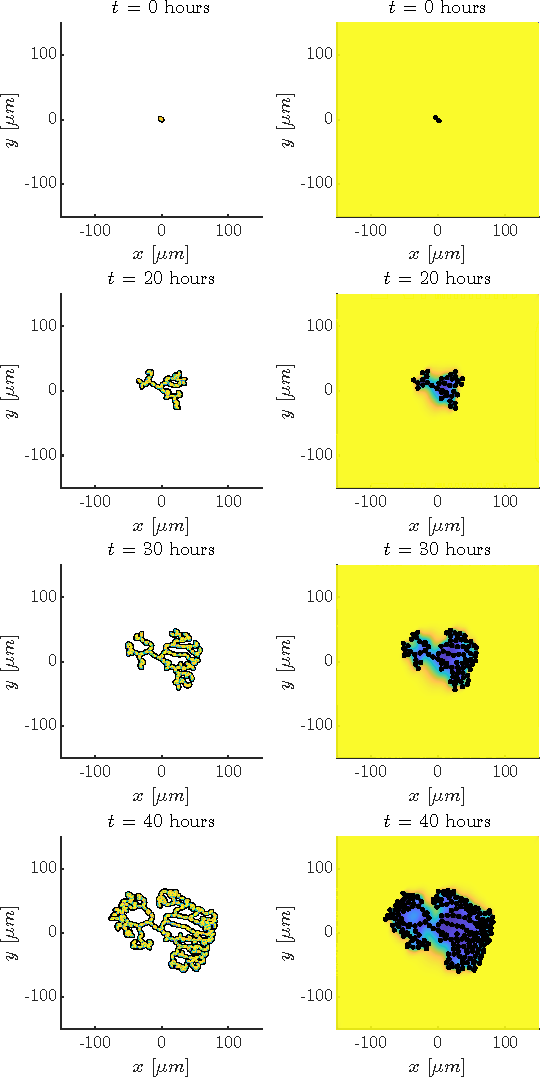
\includegraphics[width= 0.7\textwidth]{
        chapter4/figures/t_all_L1_0o10_L2_5o00_L3_5o00_L4_0o50_L5_1o00_L6_3o00_L7_0o50.pdf}
    \caption{A cell colony with parameter values given by
             $\lambda_1 = 0.1$,  
             $\lambda_2 = 5.0$, 
             $\lambda_3 = 5.0$, 
             $\lambda_4 = 0.5$, 
             $\lambda_5 = 1.0$, 
             $\lambda_6 = 3.0$, 
             $\lambda_7 = 0.5$. 
             On the left we have the biomass field, the nutrient field is on the right.}
    \label{fig:colony1}
\end{figure}

\begin{figure}[!htb] %Change this to [p] maybe ?
    \centering
    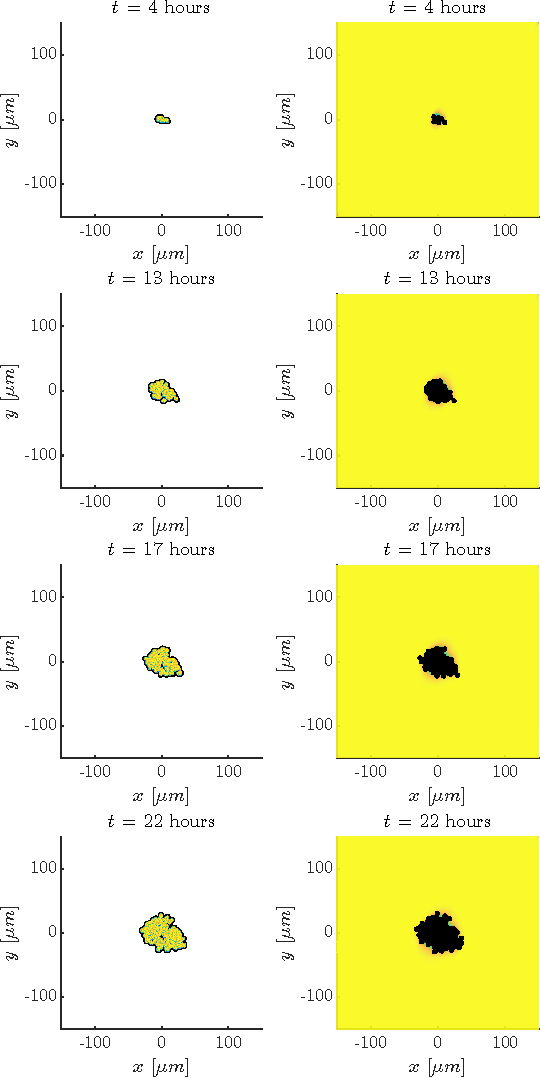
\includegraphics[width= 0.7\textwidth]{
        chapter4/figures/t_all_L1_0o10_L2_5o00_L3_5o00_L4_0o50_L5_0o10_L6_0o70_L7_0o73.pdf}
    \caption{A cell colony with parameter values given by
             $\lambda_1 = 0.1$,  
             $\lambda_2 = 5.0$, 
             $\lambda_3 = 5.0$, 
             $\lambda_4 = 0.5$, 
             $\lambda_5 = 0.1$, 
             $\lambda_6 = 0.7$, 
             $\lambda_7 = 0.73$. 
             On the left we have the biomass field, the nutrient field is on the right. 
             The aspect ratio is $\lambda_7 = 5.5/7.5 = 0.73$.}
    \label{fig:colony2}
\end{figure}

\begin{figure}[!htb] 
    \centering
    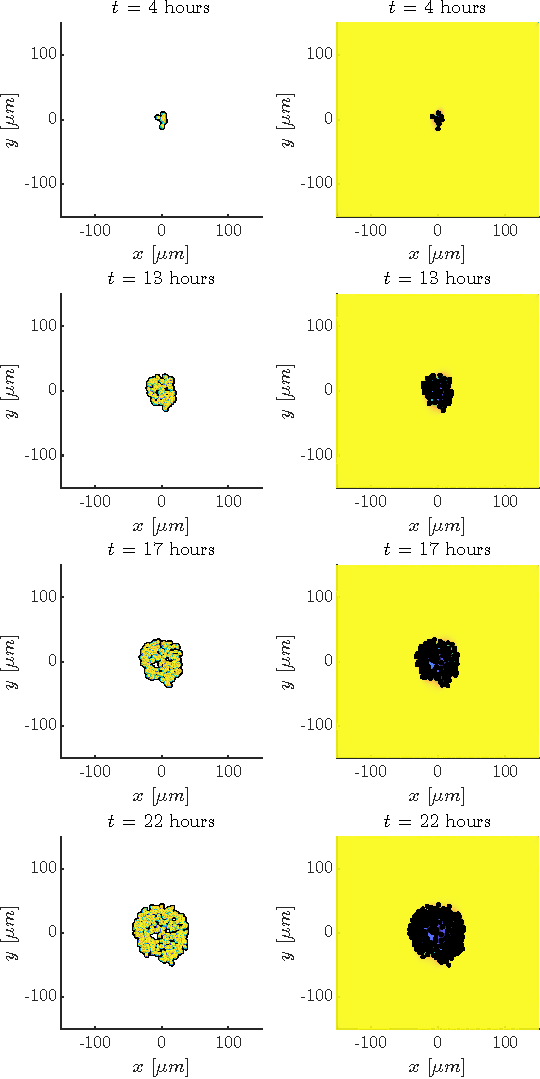
\includegraphics[width= 0.7\textwidth]{
        chapter4/figures/t_all_L1_0o10_L2_5o00_L3_5o00_L4_0o50_L5_1o20_L6_0o70_L7_0o60.pdf}
    \caption{A cell colony with parameter values given by
             $\lambda_1 = 0.1$,  
             $\lambda_2 = 5.0$, 
             $\lambda_3 = 5.0$, 
             $\lambda_4 = 0.5$, 
             $\lambda_5 = 1.2$, 
             $\lambda_6 = 0.7$, 
             $\lambda_7 = 0.6$. 
             Biomass on left and nutrient field on the right.}
    \label{fig:colony3}
\end{figure}

\begin{figure}[!htb]
    \centering
    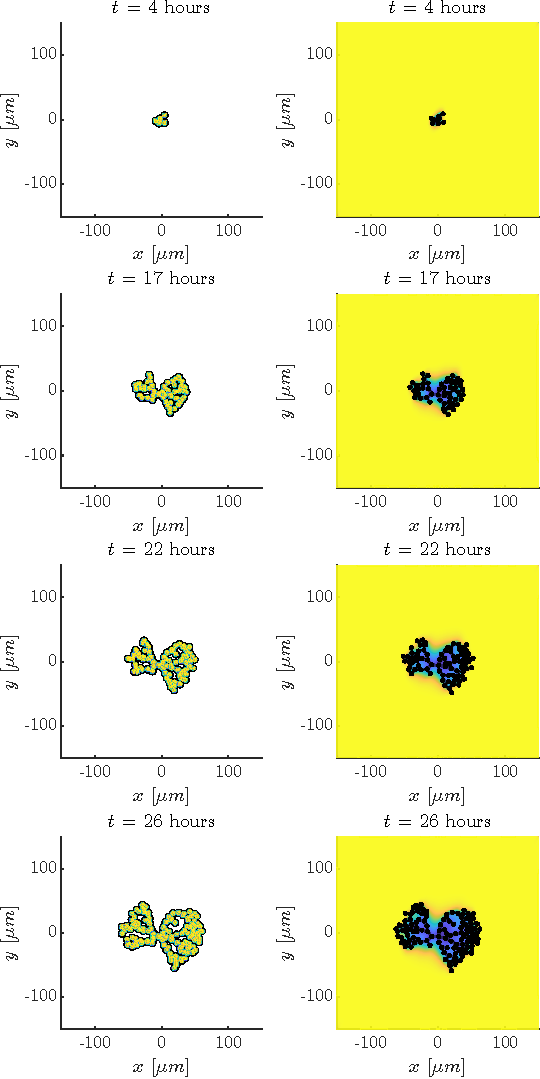
\includegraphics[width= 0.7\textwidth]{
        chapter4/figures/t_all_L1_0o10_L2_5o00_L3_5o00_L4_0o50_L5_1o60_L6_0o90_L7_0o95.pdf}
    \caption{A cell colony with parameter values given by
             $\lambda_1 = 0.1$,  
             $\lambda_2 = 5.0$, 
             $\lambda_3 = 5.0$, 
             $\lambda_4 = 0.5$, 
             $\lambda_5 = 1.6$, 
             $\lambda_6 = 0.9$, 
             $\lambda_7 = 0.95$. 
             Biomass on left and nutrient field on the right.}
    \label{fig:colony4}
\end{figure}

\begin{figure}[!htb]
    \centering
    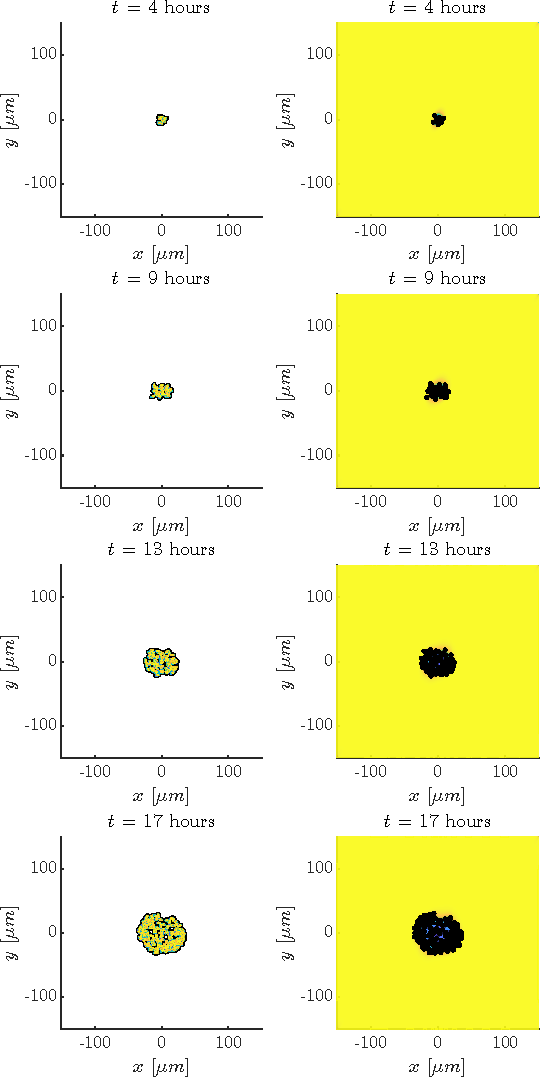
\includegraphics[width= 0.7\textwidth]{
        chapter4/figures/t_all_L1_0o10_L2_5o00_L3_5o00_L4_0o50_L5_1o60_L6_0o70_L7_0o50.pdf}
    \caption{A cell colony with parameter values given by
             $\lambda_1 = 0.1$,  
             $\lambda_2 = 5.0$, 
             $\lambda_3 = 5.0$, 
             $\lambda_4 = 0.5$, 
             $\lambda_5 = 1.6$, 
             $\lambda_6 = 0.7$, 
             $\lambda_7 = 0.5$. 
             Biomass on left and nutrient field on the right.}
    \label{fig:colony5}
\end{figure}


\section{First numerical experiment: \\ \textit{Compactness verus cell aspect ratio}}\label{sec:numExp1}
In the first numerical experiment, we vary the cell aspect ratio, $\lambda_7$,
whilst maintaining $\lambda_1 = 0.1$, $\lambda_2 = 5.0$, $\lambda_3 = 5.0$, $\lambda_4 = 0.5$, $\lambda_5 = 1.0$, 
and $\lambda_6 = 1.0$. The goal is to explore how the cell aspect ratio, $\lambda_7$, affects the overall 
colony compactness $C(t)$. The values of the mobility, $\lambda_5$, and metabolic rate, $\lambda_6$, are set to a standard 
value of $1.0$, however, a comprehensive future study should investigate how these affect the relationship
between compactness and cell aspect ratio.
\\

In figure \ref{fig:compactnessAndMu_varyAR}, the average compactness over time 
is plotted in green for cell aspect ratios of $0.4$ (elongated), $0.5$, $0.7$ and $1.0$ (circular). 
The yellow filled in area represents the $1.0 \sigma$ confidence interval for the sample 
size of $N_{\textrm{ensemble}} = 6$. This means that, running the simulation at random,
we would be approximately $68.2 \%$ sure that the compactness would lie in this range.
Of course, this confidence interval could be tightened by 
taking a larger ensemble size, $N_{\textrm{ensemble}} \gg 6$ if supercomputing 
resources are available to the user. The value of $N_{\textrm{ensemble}} = 6$ is chosen 
here due to the MSI laptop used having $6$ workers, but a larger value could 
be selected even on this hardware at the cost of multiplying the run time.
\\

As expected, the compactness more or less increases over time for all simulations, 
however figure \ref{fig:averageCompactnessComparison_varyAR} shows that the ensemble average
compactness,
$\bar{C}(t)$, grows exponentially for higher aspect ratios (approaching circular), 
and for lower aspect ratios it seems to taper off and reach a local maximum 
in the case of $\lambda_7 = 0.4$. This suggests the counter-intutitive 
conclusion that, for the parameter selection given, more circular cells 
derive more a branched colony. This is 
evinced in figures \ref{fig:compactnessSingleInstance1.0} and 
\ref{fig:compactnessSingleInstance0.5}, which shows 
the colony itself (as insetted plots) as the compactness increases for 
$\lambda_7 = 1.0$ and $\lambda_7 = 0.5$, respectively. 
\\

In figure \ref{fig:compactnessSingleInstance1.0}, 
at $t = 35$ hours, the compactness exceeds $20.0$ and 
the colony takes on a branched shape. Conversely, in figure \ref{fig:compactnessSingleInstance0.5}, 
the compactness never exceeds $10.0$. In fact, 
a circular shaped colony with comparitively lower compactness appears 
to emerge from the overall dynamics which is a suprising finding. 
This appears to be supported by the ensemble averages shown in figure 
\ref{fig:averageCompactnessComparison_varyAR}, in which
colonies with lower aspect ratio ultimately
reach a lower compactness perhaps due to emergent circularity.
\\

This seems to go against the linear logic that a higher aspect ratio indicating circular cells 
should lead to a more circular colony. The paradox can be resolved 
when we interpret the model in terms of the nominal area of each cell. 
The area of a circle of radius $0.5 \times 7.5 \ \mu m$ is about $44.2 \ \mu m^2$,
whereas the area of an ellipse is $\pi pq = \pi \times 3.75 \ \mu m \times 0.4 \times 3.75 \ \mu m =
17.7 \ \mu m^2$. The ratio of the areas is precisely $\lambda_7$ ($0.4$ in the most elongated case), which 
means that the circular cell is $2.5$ times the area of the elongated cell.
Note that we are talking about the fully grown size which I have previously characterised
by the nominal cell length $L_0 = 7.5 \ \mu m$.
\\

Interpreting this biologically, larger cell areas consume more nutrient leading
to a nutrient deficit which induces more a more branched growth regime having higher 
compactness. Conversely, lower cell areas consume less nutrient leading 
to increased crowding and the emergence of colony scale circularity.
\\

Another observation which suggests the need for further experimentation is 
the qualitative difference between the ensemble average compactness of 
$\lambda_7 = 0.4, 0.5, 0.7$ and $1.0$ demonstrated in figure \ref{fig:averageCompactnessComparison_varyAR}.
The growth curve for $\lambda_7 = 1.0$ appears to be roughly exponential,
whereas, the growth curve for $\lambda_7 = 0.4$ is almost logarithic.
How we classify the curves qualitatively is arbitrary,
but the comparison at the very least points to a qualitative 
difference between the two ends of the scale of $\lambda_7$. A question 
that could noew be posed to biologists is whether there is a critical 
value at which this transition occurs. Given supercomputing 
time, this model may indeed produce a hypthosis regarding a critical value of $\lambda_7$,
which could be tested experimentally. It may also be the case that over a large enough 
time scale we would see branching behaviour even for low values of $\lambda_7$
which would indicate two turning points: a local maximum followed by a local minium after which 
the compactness increases at an increasing rate. This ``double-ascent" if 
it were found could also be operationalisable.


\begin{figure}[!htb]
    \centering
    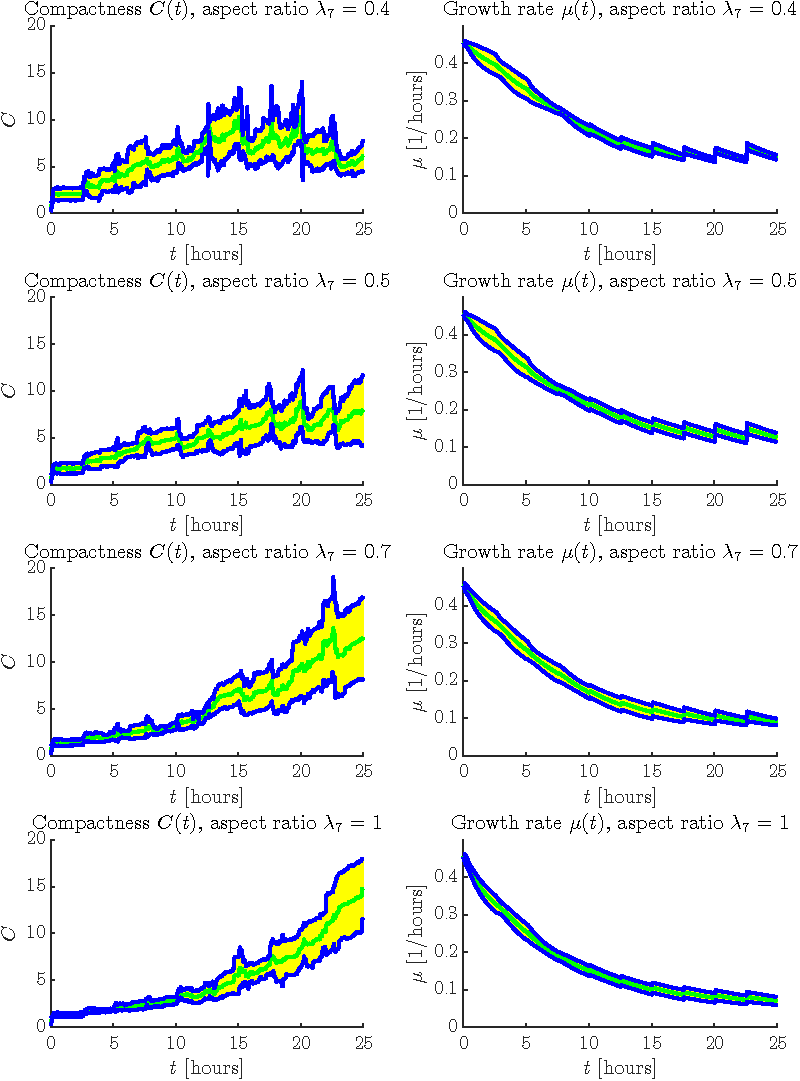
\includegraphics[width= \textwidth]{
        chapter4/figures/Comp_all_ar_EnsembleSize_6o0_L1_0o10_L2_5o00_L3_5o00_L4_0o50_L5_1o00_L6_1o00_L7_0o40.pdf}
    \caption{The colony compactness and growth rate for 
             $\lambda_1 = 0.1$,  
             $\lambda_2 = 5.0$, 
             $\lambda_3 = 5.0$, 
             $\lambda_4 = 0.5$, 
             $\lambda_5 = 1.0$, 
             $\lambda_6 = 1.0$, 
             $\lambda_7 = 0.4, 0.5, 0.7, 1.0$ and an ensemble size of $6$.}
    \label{fig:compactnessAndMu_varyAR}
\end{figure}

\begin{figure}[!htb] %Change this to [p] maybe ?
    \centering
    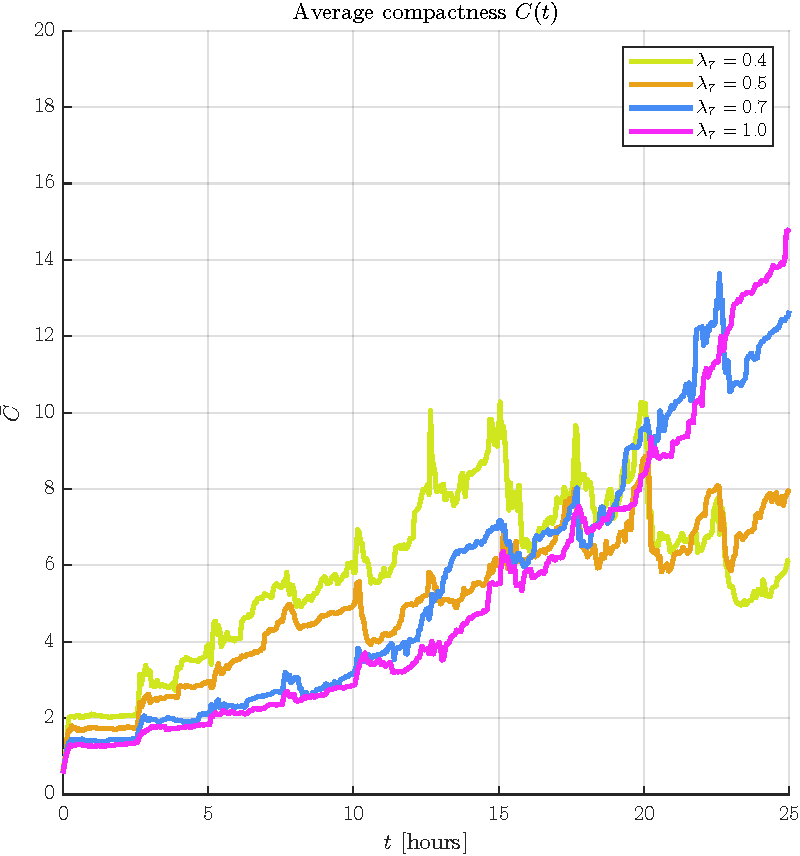
\includegraphics[width= \textwidth]{
        chapter4/figures/Comp_average_actness_EnsembleSize_6o0_L1_0o10_L2_5o00_L3_5o00_L4_0o50_L5_1o00_L6_1o00_L7_0o40.pdf}
    \caption{The average colony compactness for
             $\lambda_1 = 0.1$,  
             $\lambda_2 = 5.0$, 
             $\lambda_3 = 5.0$, 
             $\lambda_4 = 0.5$, 
             $\lambda_5 = 1.0$, 
             $\lambda_6 = 1.0$, 
             $\lambda_7 = 0.4, 0.5, 0.7, 1.0$ and an ensemble size of $6$.}
    \label{fig:averageCompactnessComparison_varyAR}
\end{figure}

\begin{figure}[!htb] %Change this to [p] maybe ?
    \centering
    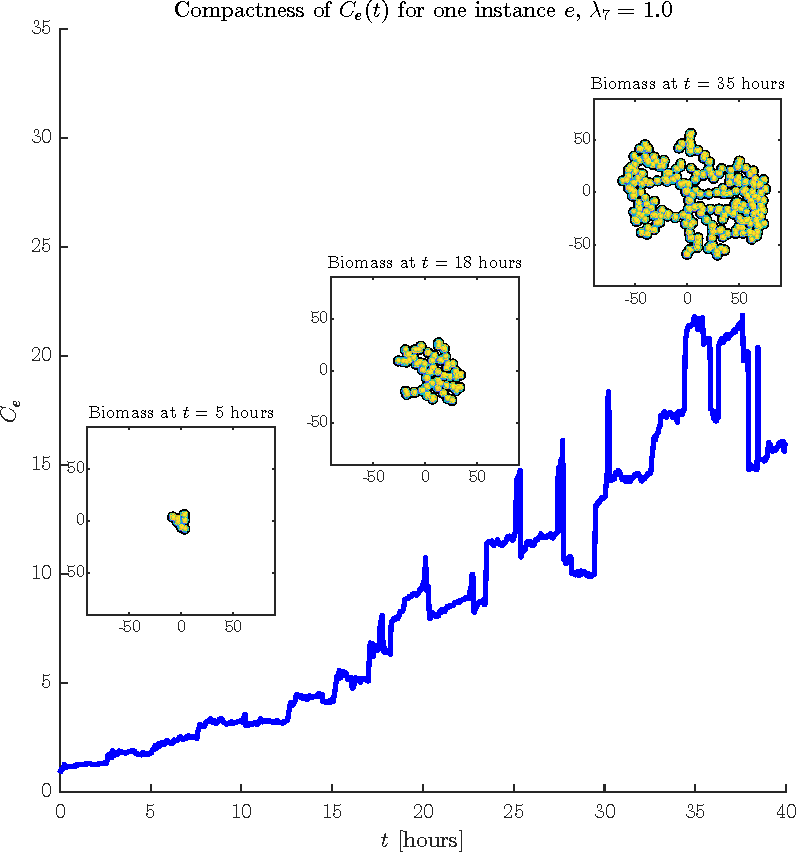
\includegraphics[width= \textwidth]{
        chapter4/figures/Inset_L1_0o10_L2_5o00_L3_5o00_L4_0o50_L5_1o00_L6_1o00_L7_1o00.pdf}
    \caption{Compactness for ensemble instance $e = 1$ and 
             $\lambda_1 = 0.1$,  
             $\lambda_2 = 5.0$, 
             $\lambda_3 = 5.0$, 
             $\lambda_4 = 0.5$, 
             $\lambda_5 = 1.0$, 
             $\lambda_6 = 1.0$, 
             $\lambda_7 = 1.0$. The inset plots show the biomass at three times for comparison 
             with compactness.}
    \label{fig:compactnessSingleInstance1.0}
\end{figure}

\begin{figure}[!htb] %Change this to [p] maybe ?
    \centering
    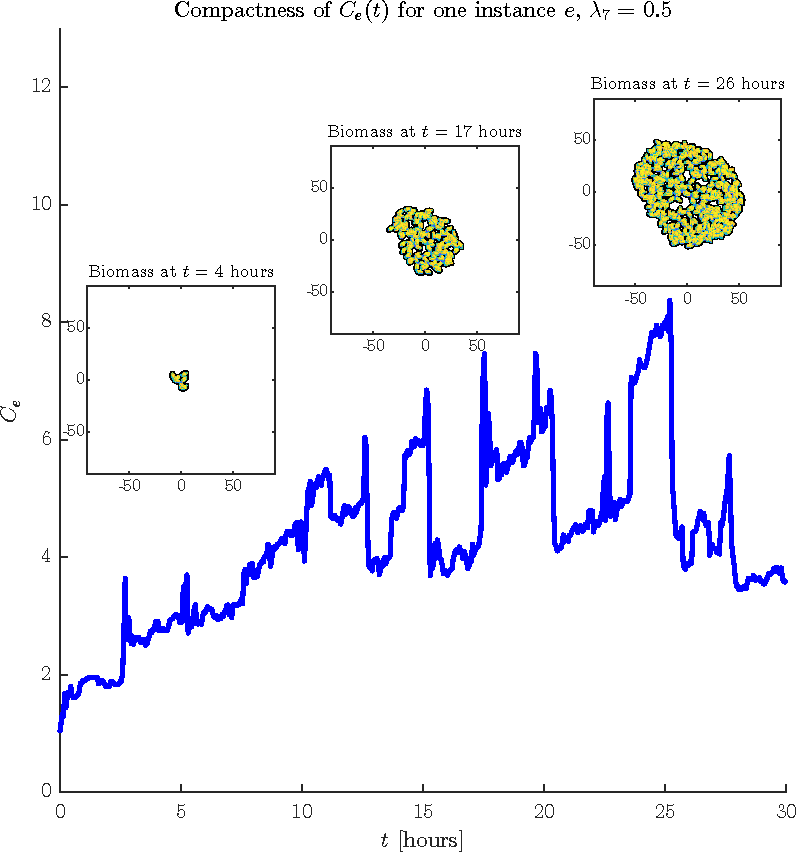
\includegraphics[width= \textwidth]{
        chapter4/figures/Inset_L1_0o10_L2_5o00_L3_5o00_L4_0o50_L5_1o00_L6_1o00_L7_0o50.pdf}
    \caption{Compactness for ensemble instance $e = 1$ and 
             $\lambda_1 = 0.1$,  
             $\lambda_2 = 5.0$, 
             $\lambda_3 = 5.0$, 
             $\lambda_4 = 0.5$, 
             $\lambda_5 = 1.0$, 
             $\lambda_6 = 1.0$, 
             $\lambda_7 = 0.5$. The inset plots show the biomass at three times for comparison 
             with compactness.}
    \label{fig:compactnessSingleInstance0.5}
\end{figure}


\section{Second numerical experiment: \\ \textit{Growth rate versus mobility}}\label{sec:numExp2}

In the second numerical experiment, the growth rate $\mu(t)$ was investigated with respect 
to its dependence on the mobility, $\lambda_5$. In all runs, the growth rate was found to be decreasing 
during times when the number of cells was fixed. At times when new cells were added in,
the growth rate would more or less instantaneously increase. 
\\

As evinced in figure \ref{fig:MuSingleInstance5.0}, adding in new cells 
could result in what appears to be a resurgence in growth rate. Of course,
further studies could focus on developing more natural ways to continuously add new cells into the 
simulation (see Chapter 4) which would allow for a smoother curve.
The fact that cells are added in at discrete intervals is a limitation of the model.
\\

Predictably, figures \ref{fig:averageCompactnessComparison_varyMobility} 
and \ref{fig:averageMuComparison_varyMobility} demonstrate 
that the growth rate decreases more slowly for colonies with higher 
mobilility, for instance $\lambda_5 = 2.5, 5.0$. Biologically,
this is likely due to the fact that new daughter cells can move more
quickly to positions of higher nutrient concentration due to a 
higher magnitude of chemotaxis. Conversely, colonies with lower mobility
deplete nutrient at the same rate however they are 
unable to move away quickly enough to maintain higher growth rate.
\\

Once again this study is somwhat limited by the hardware used. 
Given more compute power, a simulation across longer time scales and 
over larger ensembles could be 
possible which could unveil more findings, in addition to 
making the current findings more conclusive.


\begin{figure}[!htb]
    \centering
    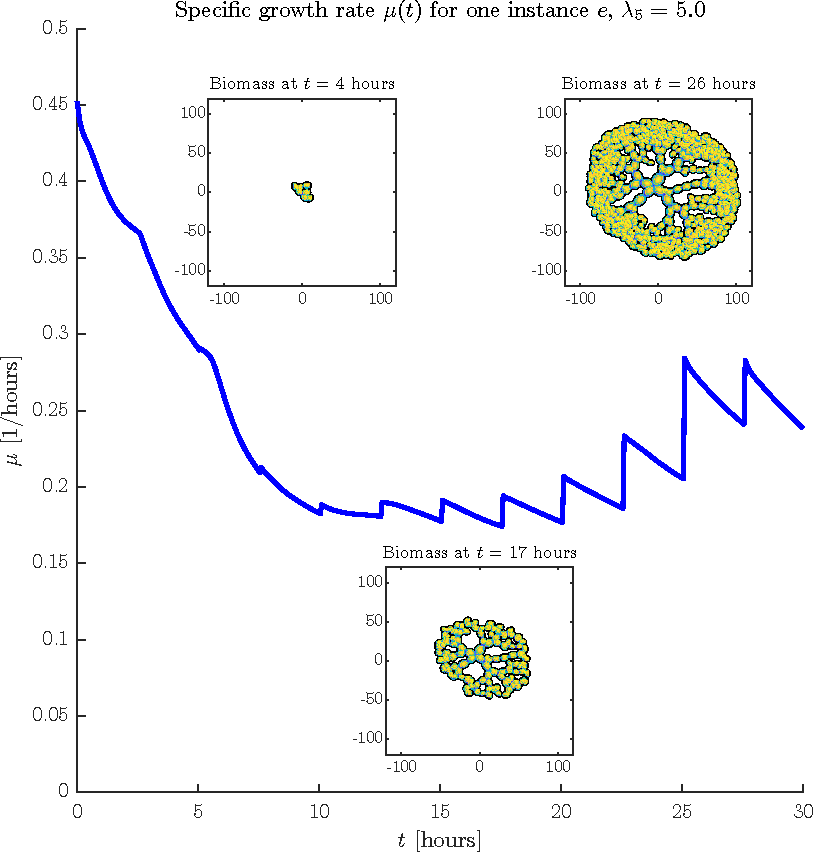
\includegraphics[width= \textwidth]{
        chapter4/figures/Inset_L1_0o10_L2_5o00_L3_5o00_L4_0o50_L5_5o00_L6_1o00_L7_0o70.pdf}
    \caption{Specific growth rate $\mu(t)$ for ensemble instance $e = 1$ and 
             $\lambda_1 = 0.1$,  
             $\lambda_2 = 5.0$, 
             $\lambda_3 = 5.0$, 
             $\lambda_4 = 0.5$, 
             $\lambda_5 = 5.0$, 
             $\lambda_6 = 1.0$, 
             $\lambda_7 = 0.7$.}
    \label{fig:MuSingleInstance5.0}
\end{figure}

\begin{figure}[!htb] 
    \centering
    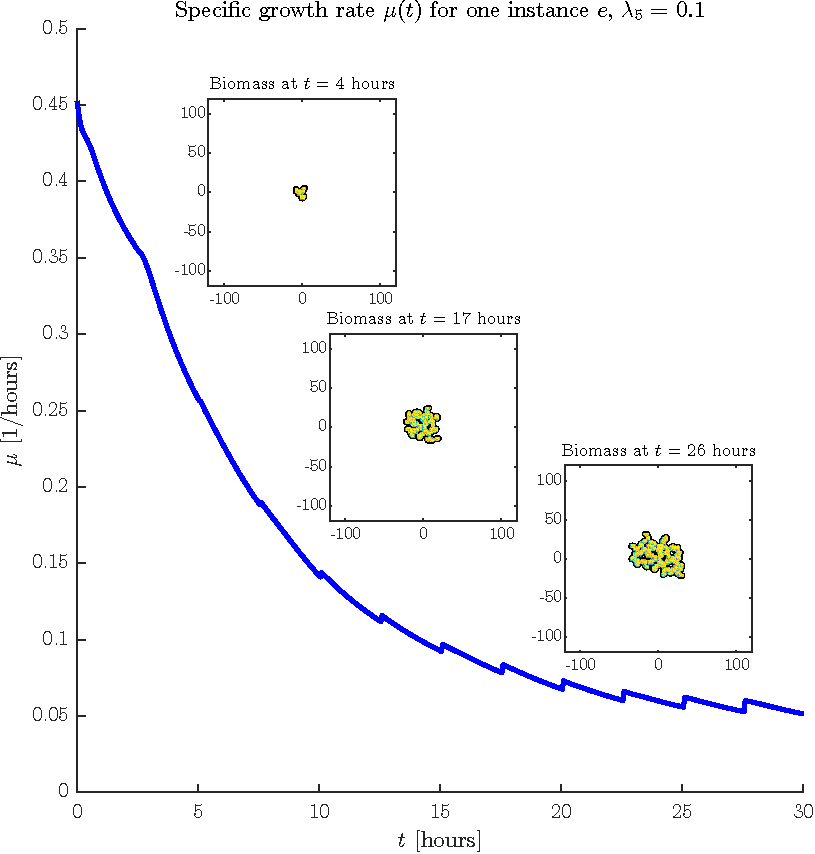
\includegraphics[width= \textwidth]{
        chapter4/figures/Inset_L1_0o10_L2_5o00_L3_5o00_L4_0o50_L5_0o10_L6_1o00_L7_0o70.pdf}
    \caption{Specific growth rate $\mu(t)$ for ensemble instance $e = 1$ and 
             $\lambda_1 = 0.1$,  
             $\lambda_2 = 5.0$, 
             $\lambda_3 = 5.0$, 
             $\lambda_4 = 0.5$, 
             $\lambda_5 = 0.1$, 
             $\lambda_6 = 1.0$, 
             $\lambda_7 = 0.7$.}
    \label{fig:MuSingleInstance0.1}
\end{figure}

\begin{figure}[!htb] %Change this to [p] maybe ?
    \centering
    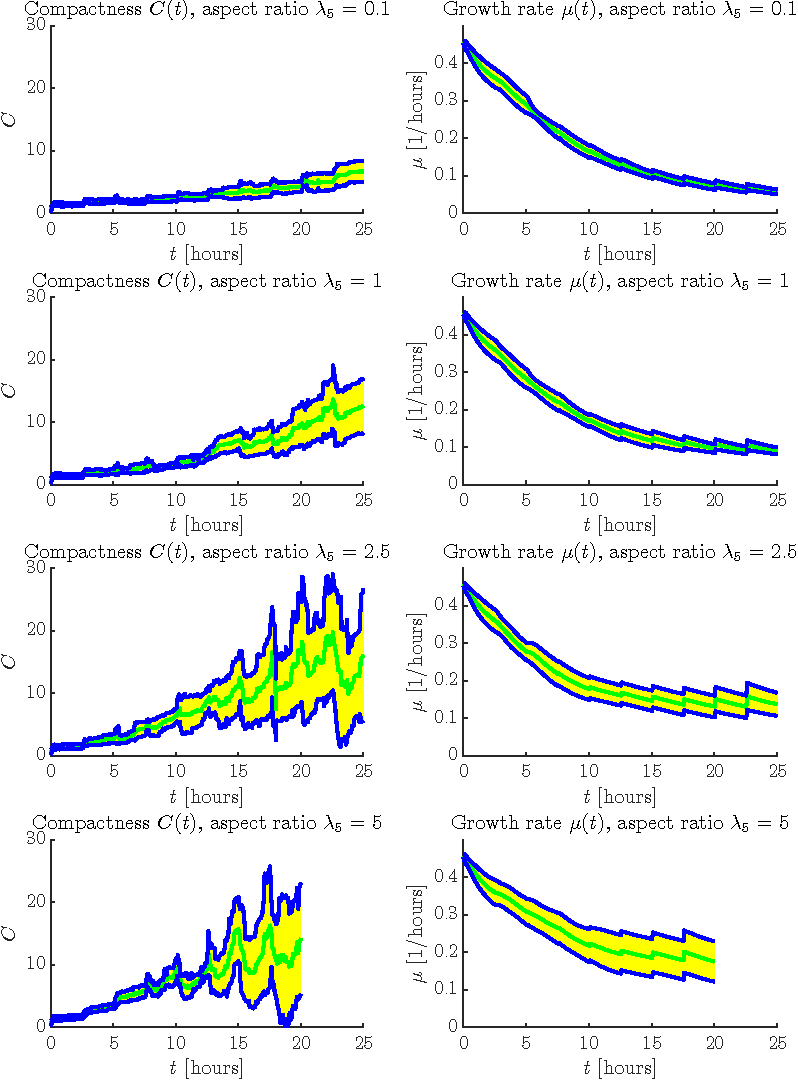
\includegraphics[width= \textwidth]{
        chapter4/figures/Comp_all_ar_EnsembleSize_6o0_L1_0o10_L2_5o00_L3_5o00_L4_0o50_L5_0o10_L6_1o00_L7_0o70.pdf}
    \caption{Compactness $C(t)$ and specific growth rate $\mu(t)$ for 
             $\lambda_1 = 0.1$,  
             $\lambda_2 = 5.0$, 
             $\lambda_3 = 5.0$, 
             $\lambda_4 = 0.5$, 
             $\lambda_5 = 0.1, 1.0, 2.5, 5.0$, 
             $\lambda_6 = 1.0$, 
             $\lambda_7 = 0.7$, and an ensemble of size $6$. Note that the bottom panels 
             could only be simulated to $t = 20$ hours due to GPU out-of-memory issues.}
    \label{fig:averageCompactnessComparison_varyMobility}
\end{figure}

\begin{figure}[!htb] %Change this to [p] maybe ?
    \centering
    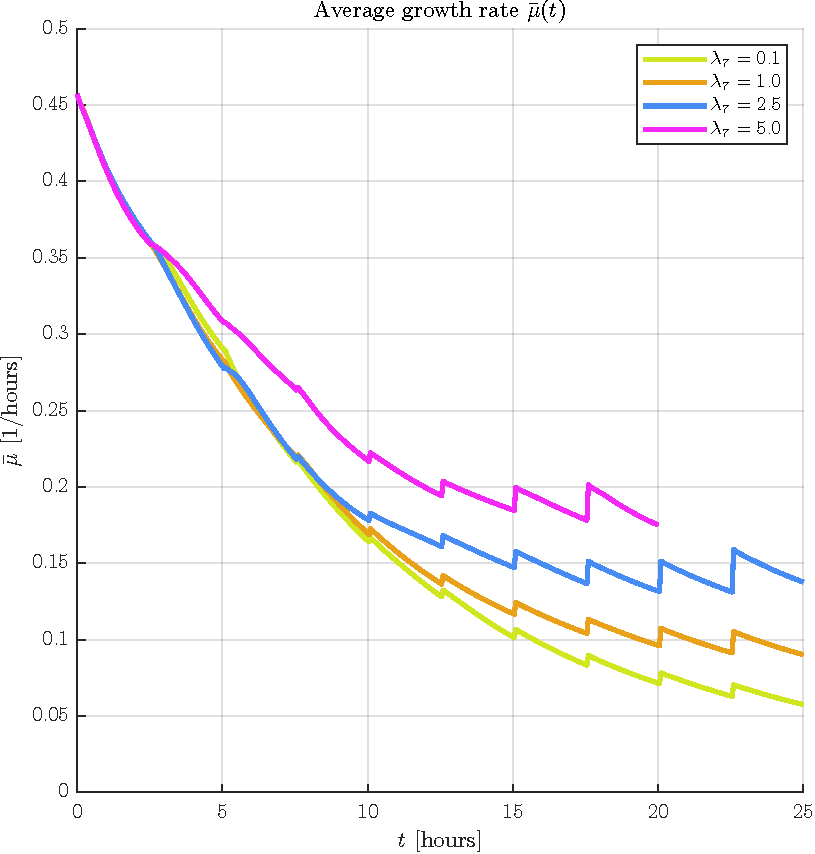
\includegraphics[width= \textwidth]{
        chapter4/figures/Average_mu_EnsembleSize_6o0_L1_0o10_L2_5o00_L3_5o00_L4_0o50_L5_0o10_L6_1o00_L7_0o70.pdf}
    \caption{Average growth rate $\mu(t)$ for 
             $\lambda_1 = 0.1$,  
             $\lambda_2 = 5.0$, 
             $\lambda_3 = 5.0$, 
             $\lambda_4 = 0.5$, 
             $\lambda_5 = 0.1, 1.0, 2.5, 5.0$, 
             $\lambda_6 = 1.0$, 
             $\lambda_7 = 0.7$, and an ensemble of size $6$. Note the plot 
             for $\lambda_5 = 5.0$ could not be completed on the aviliable hardware
             due to GPU out-of-memory.}
    \label{fig:averageMuComparison_varyMobility}
\end{figure}


\section{Summary: \\ \textit{Uncovering different growth regimes}}

Overall, the model has successfully demonstrated the ability 
to image different growth regimes of Baker's yeast morphology.
The primary strength of the model is its versalitlity:
it can model yeast morphology in both a nutrient deficit (small $\lambda_6$)
and a nutrient rich (large $\lambda_6$) case, wherein 
different qualitative behaviour is derived. 
\\

The hope is that this type of algebraic modelling of cell colonies 
can be generalised to cancer morphology. It is 
my prediction that the model, when outfitted 
to a 3D setting with access to nutrient sources such as blood 
vessels could produce fascinating findings which 
could motivate further \textit{in vitro} or perhaps even 
\textit{in vivo} experiments. One possible application is 
to tumour spheroids. In this instance, 
the model could be promoted to a 3D model which 
is not a conceptual leap but may prove to be 
a formidable computational task. Furthermore, the model could even 
be coupled to other fields,
such as electromagnetic fields. 